% Chapter 3
\chapter{Challenges and overview}\label{ch:concepts} 
\minitoc% Creating an actual minitoc
\bigskip

This chapter describes the main challenges, problems addressed, and assumptions made in this thesis related to anomaly detection in each of the system data sources. We position the methods developed in this thesis in the more general AIOps platform and provide an overview of the solution.

\section{Anomaly detection challenges in distributed software systems}
\label{ch:concepts:sec:anomalydetectionindistributedsoftwaresystems}
Several challenges that hinder the anomaly detection include training a model to capture every possible normal behavior, existence of anomalies from malicious adversaries, evolving normal behaviour, absence of labeled data, and high noise. 

The complex nature of the anomaly detection problem translates some of the detection challenges to the domain of distributed software systems.

\begin{itemize}
    \item \textbf{Low prediction rate.} Anomalies are rare events. It is challenging to identify all of them. Numerous normal instances are wrongly reported as anomalies while sophisticated anomalies are missed out. Although extensive studies have been carried out~\cite{liu2008isolation,breunig2000lof}, a large number of false positives exist in real-world datasets~\cite{du2017deeplog,campos2016evaluation,ruff-etal-2019-self,ruff2019deep}. Large distributed systems such as the cloud are constantly prone to new infrastructure and software updates and varying levels of load, noise, and users~\cite{zhang2015rapid}. For example, a system upgrade often generates novel log messages, changes the "normal" metric behavior, and most likely generates a different trace~\cite{zhang2019robust,nedelkoski2020selftracing}. In this regard, the data continuously evolve and thus the current normal behaviour may be outdated in the future. This creates a challenging environment for modeling of the normal behavior, which is crucial for anomaly detection.
    \item \textbf{Anomaly detection in high-dimensional data.} Anomalies often exhibit evident abnormal characteristics in a low-dimensional space, yet become hidden and unnoticeable in a high-dimensional space. Identifying high-order, nonlinear, and heterogeneous feature interactions and couplings may be essential in high-dimensional data. It is still a major challenge for anomaly detection. In addition, it is challenging to detect anomalies from instances that may be dependent on each other, e.g., by temporal, spatial, graph-based, and other interdependency relationships~\cite{pang2020deep}. These properties are particularly valid for log and trace data in distributed systems. Logs, as text data, often are represented as high-dimensional data~\cite{mikolov2013distributed}, while traces have an inherit graph-based relationship between the spans (representing services). 
    \item \textbf{Anomaly detection in noisy data.} Numerous anomaly detection methods assume that the given labeled training data are clean, which can be highly vulnerable to noisy instances that are mistakenly labeled by the opposite class label. For example, in training data collected from a distributed system, it is often assumed that all data are normal. However, with a high probability, anomaly samples exist in the training data, which can contaminate and degrade the model performance. Therefore, the models should be robust to such unknown deviations~\cite{du2019robust}.
    \item \textbf{Detection of complex anomalies.} Current methods mainly focus on detection of anomalies from single data sources, while various applications require detection of anomalies with multiple heterogeneous data sources, e.g., multidimensional data, graph, and text data. A main challenge is that some anomalies can be detected only when considering two or more data sources~\cite{pang2020deep}. Similar anomalies exist in distributed systems. For certain anomalies, no indication of the failure exists in the logs and no considerable change in the execution path in the traces is observed when the system operates in a degradation state. 
\end{itemize} 

For all observability components in distributed software systems, the large amounts of false-positive alarms are a major obstacle for using them in real-world production environments~\cite{meng2019loganomaly}. Detection of anomalies and alerting enable a system to report when something is broken or degraded. Notifying an operator is costly. When the alerts occur too frequently, operators second-guess, skim, or even ignore incoming alerts as they classify them as false positives (alarms). Sometimes even real treats masked by the noise of alarms are ignored. Therefore, effective anomaly detection and alerting systems have good signals and low noise or low rates of false alarms.

\begin{figure}[!t]
     \centering
     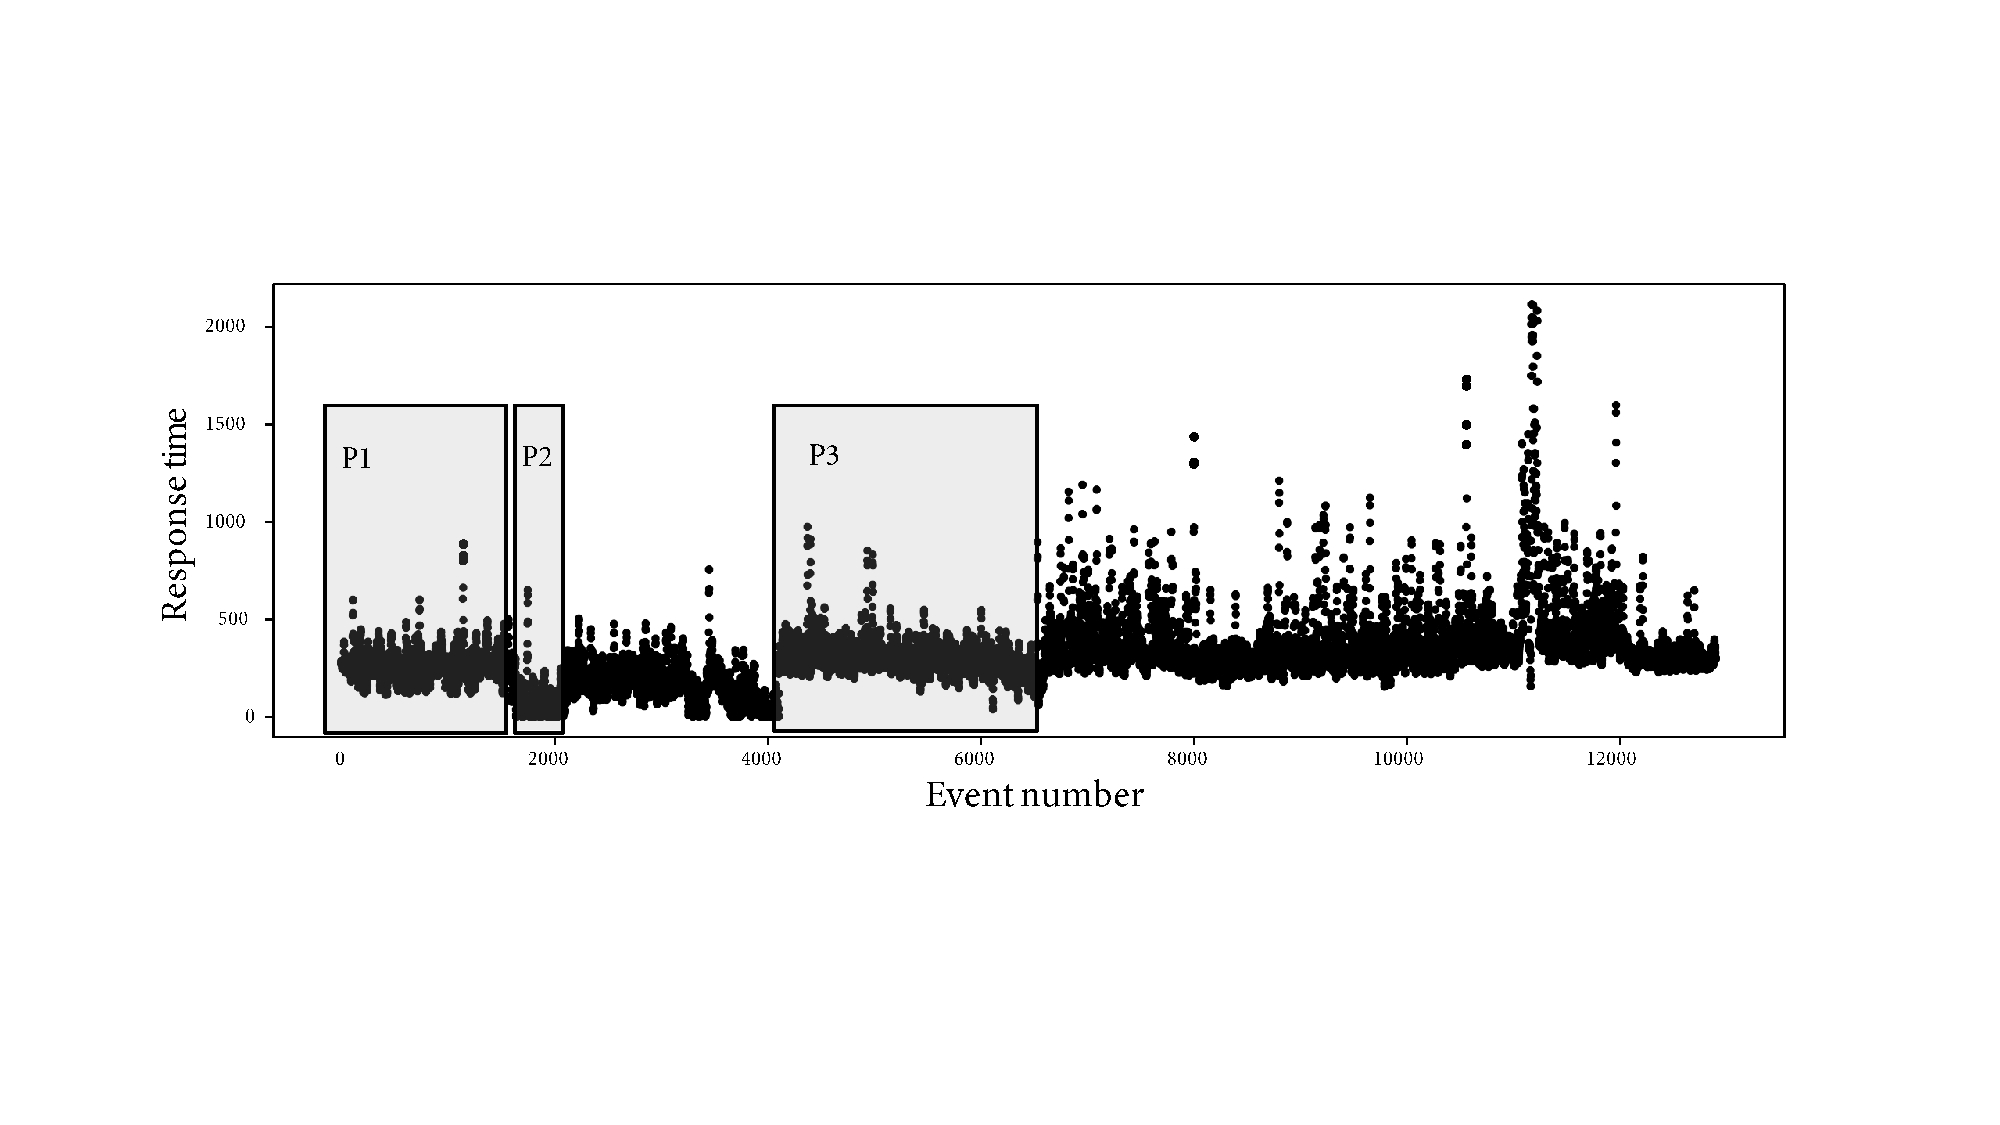
\includegraphics[width=1.0\textwidth]{gfx/chap3/multipledistributions.pdf}
     \caption{Multiple distributions representing the normal system behavior in metric data.}
     \label{fig:multipledistributions}
\end{figure}

\subsection{Metric data}
\label{ch:concepts:sec:anomalydetectionindistributedsoftwaresystems:subsec:metric}
In metric data from a distributed system, several challenges arise, including the lack of labeled data, concept drift, and concept evolution. Other major sources of difficulties emerge owing to the low signal-to-noise ratio, multiple frequencies and multiple distributions, large number of distinct time series generated by microservice applications, and concept drifts. The signal-to-noise ratio is typically low as numerous different components affect the response time of microservices such as switches, routers, memory capacity, CPU performance, programming languages, thread and process concurrency, bugs, and volume of user requests. Multiple frequencies are correlated with system and user behaviors as request patterns are different, e.g., from hour to hour due to business operation hours, from day to day due to system maintenance tasks, and from month to month due to cyclic patterns. Some of these challenges are illustrated in Figure~\ref{fig:multipledistributions}. The response time metric from a cloud service has a high level of noise ([0 ms, 2000 ms]), several distributions changing over time (P1, P2, and P3), representing the normality of the system, and additional small uptrend. 

These are stochastic properties that introduce uncertainty during the modelling phase. An additional property of metric time series inherent from time series data in general is the sequential dependence of the data points. Similar data points in the time series upon rearrangement represent different system behaviours. For example, a gradually increasing pattern, if flipped horizontally, will be a gradually decreasing pattern. The values of the data points used to form these patterns can be equal or similar; however, they reflect opposite system states. Therefore, models that aim to learn patterns from such time series need to consider the stochastic and sequential properties. 

\begin{table}[htbp]
\centering
\caption{Examples of evolving, noisy, and new log messages.}
\label{tab:evolutionlogs}
\resizebox{0.9\textwidth}{!}{%
\begin{tabular}{l|l}
\hline
Case                       & \multicolumn{1}{c}{Log messages}                                                                                                                           \\ \hline
\multirow{2}{*}{Evolution} & Faking execution of cmd: \%s"                                                                                                                              \\
                           & Faking execution of cmd (subprocess): \%s"                                                                                                                 \\ \hline
\multirow{2}{*}{Noise}     & \begin{tabular}[c]{@{}l@{}}While synchronizing instance power states, two instances \\ in the database and one instance on the hypervisor were found.\end{tabular} \\
                           & \begin{tabular}[c]{@{}l@{}}While synchronizing instance power states, two instances\\ were found in the database.\end{tabular}                                    \\ \hline
New                        & Loaded extension: binding-extended                                                                                                                         \\ \hline
\end{tabular}
}
\end{table}


\subsection{Log data}\label{ch:concepts:sec:anomalydetectionindistributedsoftwaresystems:subsec:log}
Developers and operators with understanding of the system can detect a problem that can be observed in the logs based on semantic reasoning. However, as explained above, owing to the massive amounts of log data, manual inspection is often infeasible.

In almost all live software systems, the log statements from their services evolve and are prone to processing noise over time. Developers may frequently modify source codes including logging statements, which in turn leads to changes to log data. Kabinna et al.~\cite{kabinna2018examining} observed that approximately 20\%-45\% of logging statements in their studied projects changed throughout their lifetime. Google’s systems have up to thousands of new log printing statements every month~\cite{xu2010system}. 

Furthermore, during collection, retrieval, and preprocessing of log data, a certain degree of noise is inevitably introduced into the original log data. For example, the noise may originate from the data collection process. In a large-scale system, numerous logs are produced by geographically distributed components separately, and then uploaded to a centralized location for further analysis. Missing, duplicated, or disordered log messages can originate from such a process (e.g., due to network errors, limited
system throughput, and storage issues).

We show examples of evolving, noisy, and new log statements in Table~\ref{tab:evolutionlogs}. In the case of evolving statements, the (subprocess) word is added for clarity. In the noisy logs, owing to the lack of instances on the hypervisor, a different print statement that shortens the message is observed. In system upgrades, often new log messages appear owing to, e.g., extensions. 

Logs are developer-written text sentences. Each developer has a specific style of programming and writing log statements~\cite{zhu2019tools}. This contributes to the inability of log analysis methods (e.g., parsing and anomaly detection) to have a standardized or more structured approach that will generalize across different datasets with minimal number of domain/system based heuristics.

These problems suggest that any method developed for log analysis needs to discard the close-world assumption, where systems are not evolving~\cite{du2019lifelong,du2017deeplog}. The methods need to address the described challenges during the design of their models. This is particularly important for organizations that use the Continue Delivery/Deployment approaches, where the environment poses larger challenges~\cite{chen2015continuous}.

\begin{figure}[!htbp]
     \centering
     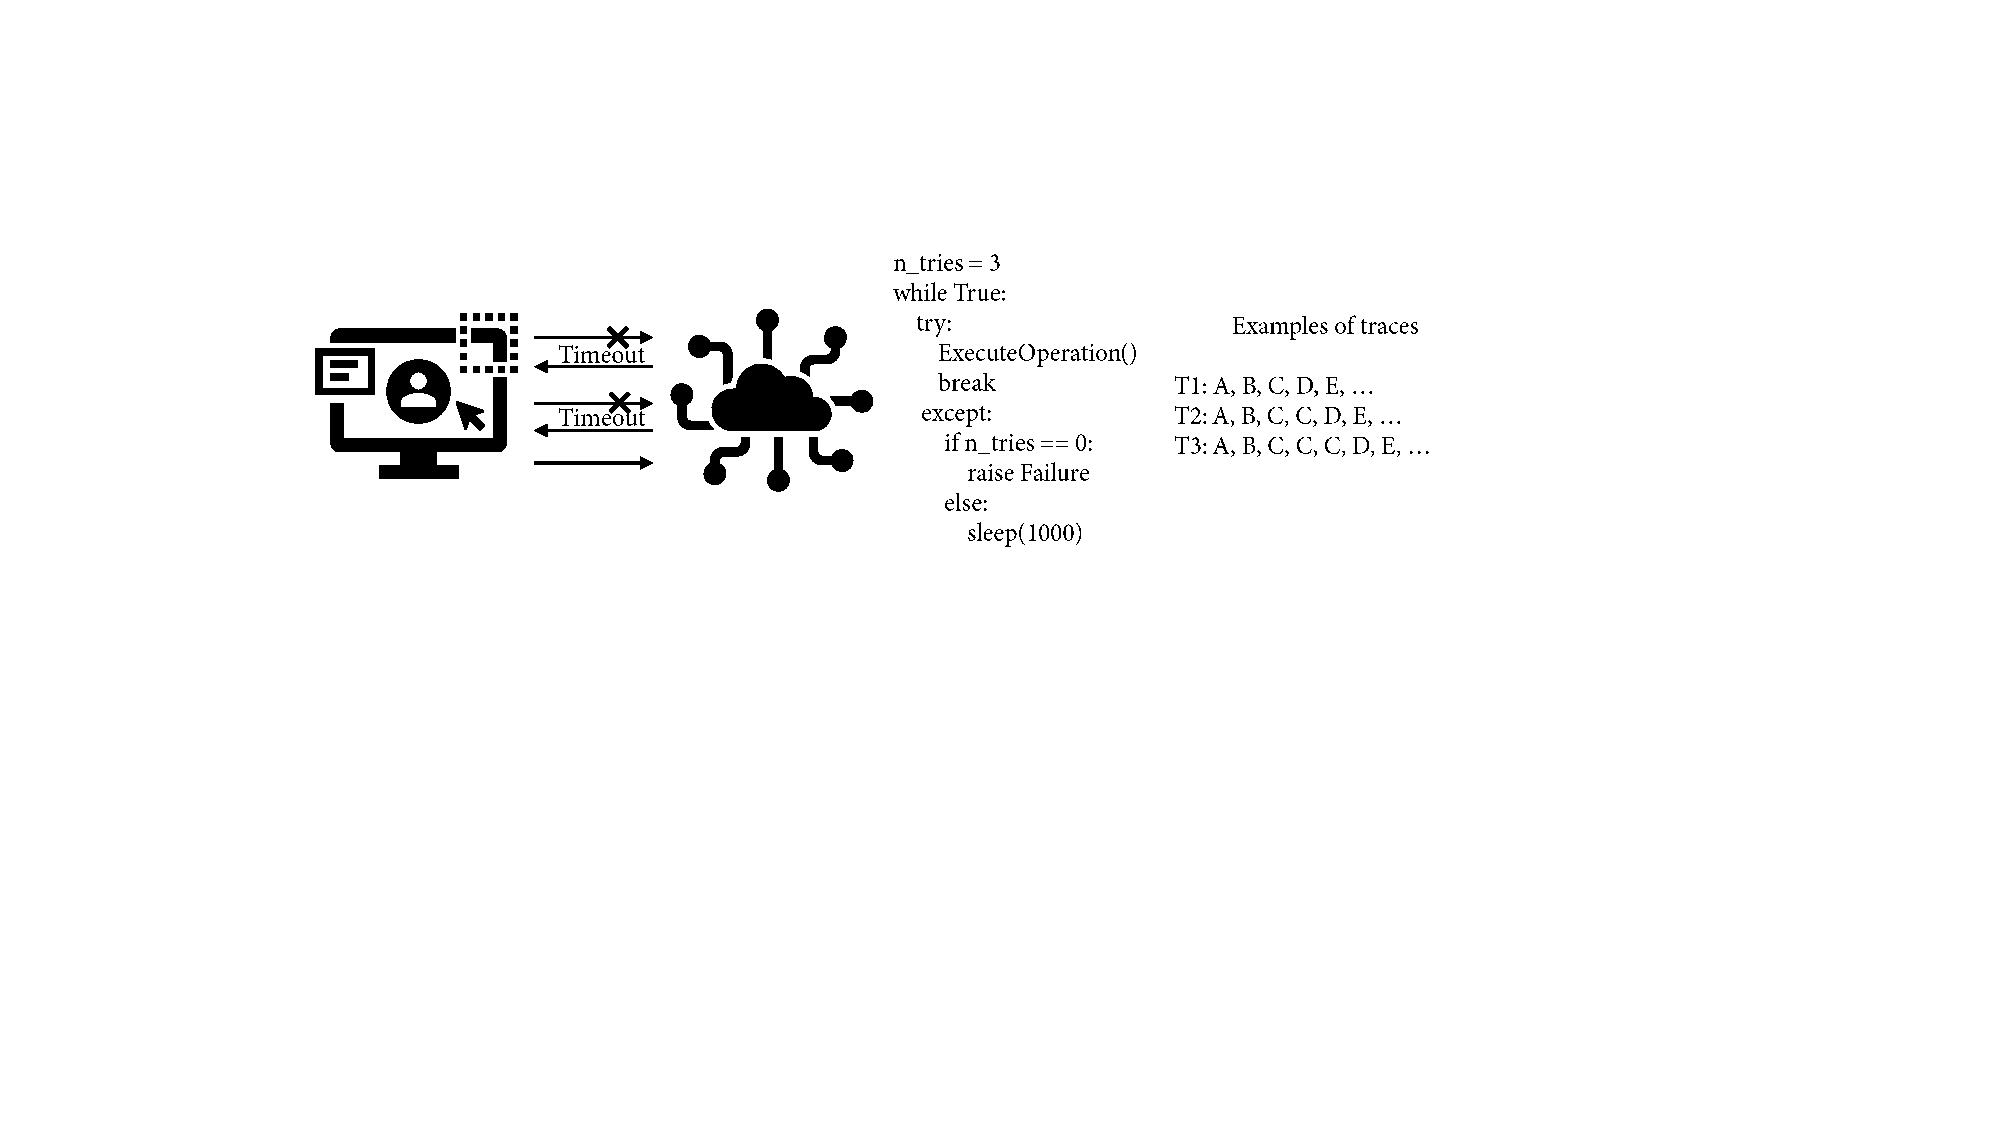
\includegraphics[width=0.99\textwidth]{gfx/chap3/traceschallenges.pdf}
     \caption{Software patterns; e.g., the retry pattern affects the running system and trace data.}
     \label{fig:tracechallenges}
\end{figure}

\subsection{Distributed tracing data}\label{ch:concepts:sec:anomalydetectionindistributedsoftwaresystems:subsec:trace}
Three important challenges exist in anomaly detection from distributed traces. They are related to the existence of noise, arbitrary lengths of the traces, and lack of labels. From these challenges, the lack of labels is a lasting problem in the task of anomaly detection in general and was described in the previous chapter.

Owing to the complex nature of the operations within a distributed environment and high noise, although the observed sequence of events may not be present in the set of observed traces, it may still be normal. Noise in the traces occurs because complex systems rely on software patterns, such as caching and load balancing, to increase the efficiency and reliability. For example, it can be a retry pattern where an operation is executed, leads to a timeout, and is performed again until completion (see Figure~\ref{fig:tracechallenges}). The noise has a strong implication for trace anomaly detection as methods need to classify traces that were not observed before as normal. 

The challenge related to the range of lengths of a trace occurs mainly owing to the existence of different requests. For example, creation of a virtual machine and creation of a storage will lead to two different traces. The novel methods for anomaly detection from distributed traces, similarly to metric and log data, are faced with the scarcity and unavailability of labels when a trace is normal or anomaly. The unsupervised learning methods are considered as obtaining labels from the systems is a challenging task. The frequent system updates and volatile environment contribute to the manifestation of new patterns, which imposes a constraint of frequent updates of the labels. This is often an expensive procedure because it assumes constant availability of a domain expert.


\subsection{Complex anomalies}\label{ch:concepts:sec:anomalydetectionindistributedsoftwaresystems:subsec:complexanomalies}
Anomalies can be complex and not always represented in all data sources. Examples of such anomalies are hidden anomalies, not reflected in all observability data, and propagated anomalies, reflected in a set of system components different than the faulty component. These anomalies may not be notified to the user through exceptions or may not be monitored~\cite{sillito2020failures}. These cases represent a high risk for system operators as they lack clues for understanding the failure and restoring the availability of services and resources~\cite{gunawi2014bugs,cotroneo2019bad,sillito2020failures}. 

According to a set of experiments~\cite{cotroneo2019bad} on OpenStack, software anomalies often cause an erratic behavior of the cloud management system, hindering detection and recovery of failures. Failures were notified to the users only after a long delay, when it is more difficult to trace back the root cause of the failure and recovery actions are more costly (e.g., reverting the database), or the failures were not notified. Anomalies are not always present in all observability components and often propagate and are detected at system components different than the root-cause component. This makes the task of debugging more challenging. Therefore, for improved diagnostics, often, a combination of highly accurate models for anomaly detection in multi-view data sources is required.

\subsection{Assumptions}
In this section, we discuss observations in each of the data components, which were treated as assumptions for the design of the practical solutions. 

\noindent\textbf{General assumptions.} Throughout this thesis and description of the methods, unless otherwise stated, we use a general assumption that all data used to create the models reflect the normal system behaviour and almost do not contain anomalies~\cite{chandola2009anomaly,ruff2020unifying,ruff2019deep}. Most of the systems operate normally, most of the time, while anomalies occur rarely~\cite{du2017deeplog,meng2019loganomaly,nedelkoski2019anomalymultimodal}. Thus, in most of the production cases, using all available data satisfies the assumption, considering that, even if anomalies are present, their number is considerably smaller than the number of normal data points. The models described in this thesis implement practices to handle such cases. 

A general assumption for most deep learning methods, also implemented in this thesis, is the existence of a sufficient amount of data representing the normal system behavior. Unless otherwise stated, anomaly labels are not accessible. These are important assumptions for the development of anomaly detection methods for distributed system data. They pose requirements for the methods to be unsupervised, which is desirable and of practical value.

Lastly, a general assumption of this thesis is that system anomalies are reflected in at least one of the three data sources. In practice, the anomaly may not be reflected in the data, but can only be found by reproduction and troubleshooting in the source code. We assume that the source code of the system is not available.

Below, we discuss assumptions considered for each of the data sources.

\begin{enumerate}
    \item \textbf{In metric data}, we assume univariate time series data (unless otherwise stated in a particular experiment). Univariate anomaly detection aims to find anomalies in each individual metric, while multivariate anomaly detection learns a single model for all metrics in the system. Univariate methods are simpler, and thus they can be more easily scaled to many metrics and large datasets~\cite{Sandilands2014}. However, the task of learning the causal relationships between the anomalies in the resulting alerts from the univariate anomaly detectors remains to be performed on a higher level of abstraction~\cite{simhon2016heuristic}. This is in line with the long-lasting research on univariate time series data~\cite{braei2020anomaly}. With multivariate methods, each added metric introduces interactions between it and all other metrics. As multivariate anomaly detection methods have to model the entire complex system, the computational cost rapidly increases with the number of modeled metrics. In addition, individual metrics need to have similar statistical behaviors for accuracy of the multivariate methods~\cite{toledano18a}.
    
    \item \textbf{Logs} are generated by a software program that follows a set of instructions to serve a request, e.g., creating a virtual machine in cloud platforms. In distributed systems, multiple such requests are served in parallel. In many systems, the logs do not contain identifiers that could chain events that serve the same requests together into a group. Often, when sorted by timestamp, such sequences of logs are lost. Therefore, in this thesis, we focus on the analysis of the collected log messages as independent instances. The log anomaly detection method detects anomalies per log message, not per sequence of log messages. 
    
    A common assumption in anomaly detection from logs is that the information of the log messages is contained in their log templates (constant parts). For example, we consider a log message "Took 20.12 seconds to build instance". The methods for log-based anomaly detection focus on detecting anomalies on "Took * seconds to build instance", without considering the variable part. This assumption is common in numerous log anomaly detection approaches ~\cite{du2017deeplog,meng2019loganomaly,zhang2019robust,du2019robust,he2017drain}. Anomalies that exist in the variable parts of the log messages (e.g., numeric values) are considered as a part of time series anomaly detection (metric data). 
    \item \textbf{For trace data}, we assume that the traces are composed of a finite number of possible spans. This implies that test traces are composed of spans observed during the modeling phase. As the spans correspond to invoked services, we consider this as a weak assumption, which is not valid only when new services are deployed. In this regard, the learned model on the traces will need to be retrained once a new service is deployed within the distributed system. 
\end{enumerate}

\section{Conceptual overview}\label{ch:concepts:sec:conceptualoverview}
To address the above challenges and consider the assumptions for anomaly detection, in this thesis, we present methods for the three observability components, metrics, logs, and traces.  
The observability and anomaly detection methods are base components of a broader-context platform referred to as AIOPs platform. We show a reference architecture in Figure~\ref{fig:aiopsplatform}, where a software system based on a distributed architecture (e.g., microservices) is deployed. 

\begin{figure}[!t]
\centerline{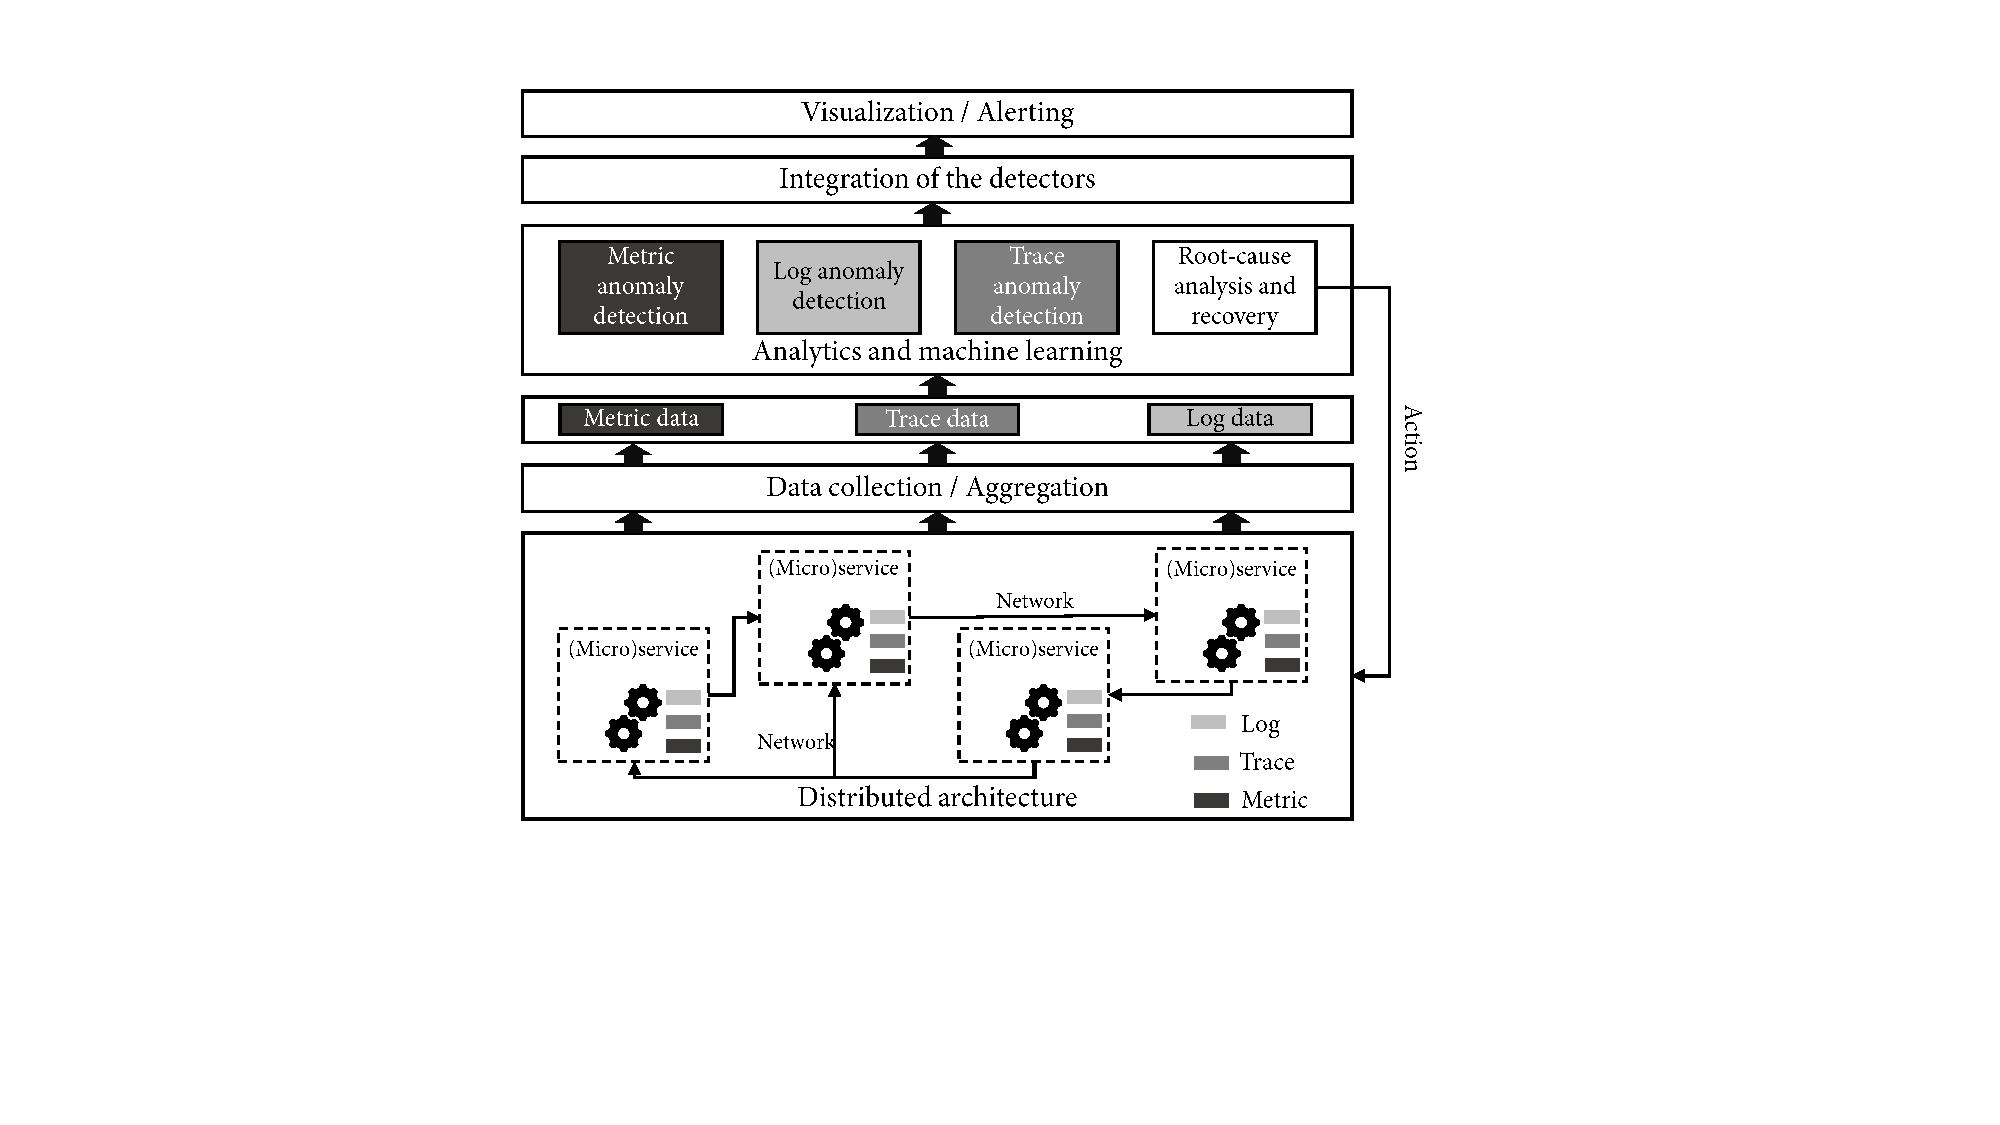
\includegraphics[scale=0.8]{gfx/chap3/aiopsplatform.pdf}}
\caption{Overall architecture of a distributed system with integrated observability components (metrics, logs, and traces) utilized by the analytic part for visualization and alerting.}
\label{fig:aiopsplatform}
\end{figure}

In every service of the distributed system, three data collection components, metrics, logs, and traces, exist. The data are then aggregated and forwarded to the analytic part. For the metric data, the aggregation is carried out per service where metrics such as CPU, memory, disk utilization, and network statistics are collected. The logs from all services are aggregated in a database with a possible separation by the service/physical host. Finally, the tracing data involve multiple hosts and services traversed while executing a request (e.g., user request). 

The data serve as a basis for the analytic and machine learning parts where several major tasks are performed. The analytic part involves preprocessing for each type of data. 

In the anomaly detection module, we consider three anomaly detectors $f_m(\mathbf{x_m})$, $f_l(\mathbf{x_l})$, and $f_t(\mathbf{x_t})$ for the metrics, logs, and traces, respectively. The input data in (1) $f_m(\mathbf{x_m})$ are a time series representing a system metric $\mathbf{x_m}={x_m^{w_m}, x_m^{w_m}, \dots, x_m^{w_m}}$, where $w_m$ is a window size, in (2) $f_l(\mathbf{x_l})$ are a system log message $\mathbf{x_l}={x_l^1, x_l^2, \dots, x_l^m}$, where $x_l^i$ are $d-$dimensional representations of the words in the log message and $m$ is the number of words, and in (3) $f_t(\mathbf{x_t})$ are a trace $\mathbf{x_t} = {x_t^1, x_t^2, \dots, x_t^k}$, where $x_t^i$ is a span and $k$ is the number of spans in the  trace. 
Each of the separate methods for anomaly detection in metrics, logs, and traces presented in this thesis is designed to mitigate the previously described challenges. Below, we present main questions derived from the challenges and methods to address them on an abstract level.

\begin{enumerate}
    \item The challenges of anomaly detection in metric data pose difficulties toward an accurate understanding of the system behavior. The major questions are related to the efficient extraction of temporal correlations within the time series, learning of multiple modes of normal behavior, noise mitigation, and description of the anomaly patterns. We address these questions aiming to improve the analysis of metric data and alert the user if there is an abnormal system behavior in the system. The core idea of the approach is to learn robust latent representations to capture normal patterns of a time series, considering both temporal dependence and stochasticity. We design the method's basis to have a variational component that provides the needed capacity of the method to learn multiple scenarios of normal system behavior and mitigate the effect of the noise and recurrent encoder and decoder networks to extract sequential features. 
    
    \item System log analysis is a lasting research topic, which, through the years, established an analysis pipeline. Traditionally, the first step in the process is to parse the unstructured log messages into structured data or extract log templates. Structured data usually refer to the constant string in each log message or the print statement. Subsequently, these templates are vectorized (e.g., count vectors~\cite{lou2010mining,xu2009detecting}) to obtain numerical representations suited for further analysis. Lastly, the log vectors are utilized as an input to the anomaly detection model. It is important that all steps in the pipeline are addressed correspondingly. Therefore, we analyze several topics including the generalization of parsing and log anomaly detection methods on unseen log messages (e.g., due to upgrades), efficient log parsing without system-dependent heuristics, and generation of learnable log vectors that are sufficiently robust to mitigate the effects of log evolution. We start with a self-supervised neural language modelling approach to log parsing. The advantage of such approach is that it replaces heuristics with learnable parameters optimized for the respective data. Concurrently, the model is designed to learn and generate log vectors, which is crucial to improve the anomaly detection~\cite{zhang2019robust}. To further improve the generalization in log anomaly detection, we describe a novel objective function and propose modification to the parsing approach. Such approach aims to learn meaningful log representations for anomaly detection, regularize against over-fitting, extract semantic knowledge from the log messages, and improve the generalization. The core principle of the method is to learn log representations in a manner to distinguish normal data from the system of interest and anomaly samples from auxiliary easily-accessible log datasets. 
    
    \item The challenges of the trace data lead to several questions, which, when addressed, have the potential to improve the anomaly detection. The research questions regarding the trace data that are addressed in this thesis are related to the modeling of traces with variable lengths, mitigation of the noise that reflects as added/missing spans form the trace, and identification of key spans within the trace, representative of the normal system behaviour, which help find the root cause of the problem. We compile the trace structure as a text sequence. This allows to utilize methods from the field of natural language processing that already tackle problems as modeling inputs with different lengths (e.g., for texts). Subsequently, to mitigate the effects of the noise, we present a task formulation based on self-supervised learning to learn the likelihood of appearance of particular span with given context spans. This enables the model to focus on particular important spans of the trace and mitigate the effects of the noise. 
\end{enumerate}

The output of each anomaly detectors at time $t$ is a label $y\in\{0,1\}$, where 0 represents a normal system behaviour, while 1 represents an anomaly.
On top of the outputs of the anomaly detection methods, a time window $w$ is utilized to aggregate the predictions for a final decision, whether an anomaly exists in the observed distributed system. Formally, the final output at a time of $t$ is $g_t(f_m, f_l, f_t, w)$, which again is 0 or 1. The main contributions of the thesis are the methods presented for metrics, logs, and traces. Finally, we analyze their integration into a framework for detection of complex anomalies.

The identified anomalies can be further employed in other AIOPs tasks. For example, together with the system topology, they are often utilized to perform a root cause analysis to identify the reason for and location of the anomaly. To complete the AIOPs loop, recovery actions need to be executed to restore a failed component or prevent further fatalities. Finally, the alerts from the anomaly detection, root cause analysis, and recovery actions are visualized to the developers, reliability engineers, and management teams to obtain better insights into the system. 
